\section{Auswertung}
\label{sec:Auswertung}
\subsection{Bestimmung des magnetischen Momentes mit Präzession}

In Tabelle \ref{tab:Präzession} sind die Werte der Umlaufdauer in Abhängigkeit von der Stromstärke $I_H$ aufgelistet.
Für die drei Messwerte pro Stromstärke wird hier mit 
\begin{equation}
  \overline{T}=\frac{1}{n} \sum_{k=1}{n} T_K
\end{equation}
der Mittelwert berechnet.
Die magnetische Flussdichte wird mit Formel \ref{eqn:magfeld} bestimmt.
Die Mittelwerte der Periodendauern werden in \ref{fig:Präzession} gegen die magnetische Flussdichte geplottet
Dazu wird lineare Regression durchgeführt, wobei die Ausgleichsgerade die Steigung $a=\qty[per-mode=fraction]{25.20956(1.21108)}{\per\second\per\tesla}$ beträgt.
Wenn Formel \ref{eqn:schwingdauer1} und \ref{eqn:Drehimpuls}zu 
\begin{equation*}
  |\vec{m}|=\frac{4 \pi^2 f L_K}{T B}
\end{equation*}
umgeformt wird, kann $a=\frac{1}{TB}$ eingesetzt werden.
Das Trägheitsmoment der Kugel wird mit Formel \ref{eqn:trägheit_kugel} $L_K=\qty{3.75e-5}{\kilo\gram\meter\squared}$. 
Damit ergibt sich dann $|\vec{m_P}|=\qty{0.18661(0.00896)}{\ampere\meter\squared}$.



\begin{table}
  \centering
  \caption{Tabelle für die Stromstärke der Helmholtz-Spulen, die drei Werte pro Stromstärke für die Periodendauer und das Mittel der drei Werte.}
  \label{tab:Präzession}
  %\sisetup{table-format=1.1, per-mode=reciprocal}
  \begin{tblr}{
      colspec = {S[table-format=1.1] S[table-format=2.2] S[table-format=2.2] S[table-format=2.2] S[table-format=2.2]},
      row{1} = {guard, mode=math},
    %  vline{4} = {2}{-}{text=\clap{$\pm$}},
    }
    \toprule
    I_H \mathbin{/} \unit{\ampere} & \SetCell[c=3]{c} T \mathbin{/} \unit{\second} & \overline{T} \mathbin{/} \unit{\second}\\%& T_2 \mathbin{/} \unit{\second} &T_3 \mathbin{/} \unit{\second} \\
    \midrule
    1 & 13.53 & 21.18 & 23.58 & 19.43\\
    1.5&17.15 & 15.40 & 17.52 & 16.69\\
    2 & 12.20 & 12.92 & 13.03 & 12.72\\
    3 &  8.55 &  9.00 &  8.73 &  8.76\\
    4 &  6.76 &  6.61 &  6.50 &  6.62\\
    \bottomrule
  \end{tblr}
\end{table}

\begin{figure}[H]
  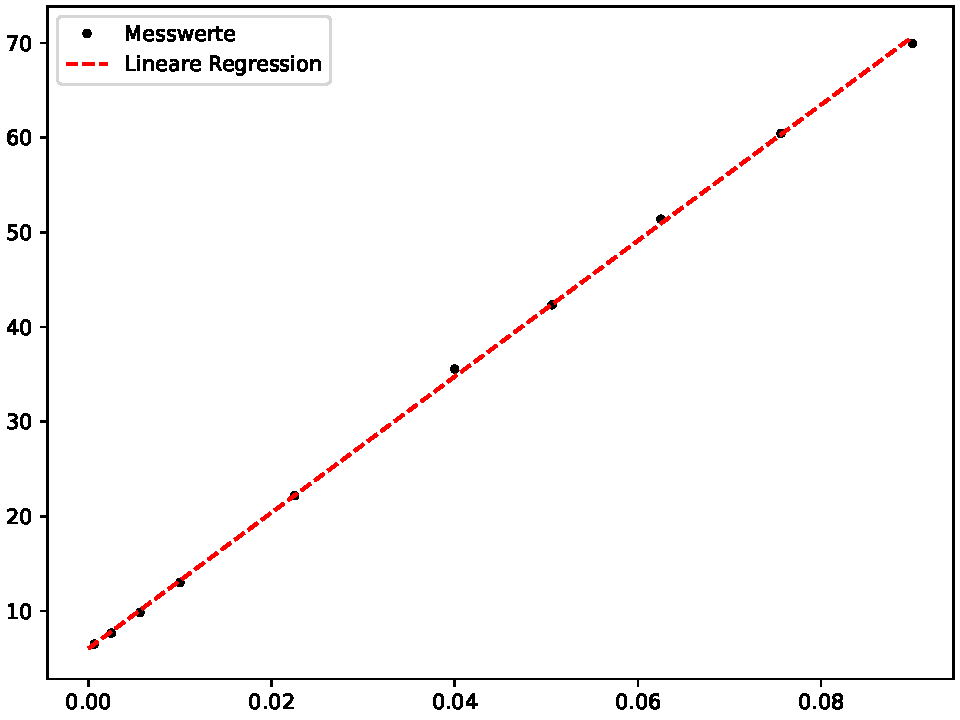
\includegraphics[width=\textwidth]{plot.pdf}
  \caption{Aufgetragen ist die gemittelte, reziproke Periodendauer in Abhängigkeit zur magnetischen Flussdichte.}
  \label{fig:Präzession}
\end{figure}

\subsection{Gravitative Methode}

\begin{table}[H]
    \centering
    \caption{Benötigte Stromstärke, damit das Drehmoment des Magnetfeldes das der Gravitation ausgleicht.}
    \label{tab:grav}
    \begin{tblr}{
        colspec={S S},
        row{1}={guard, mode=math},}
        \toprule
        r\mathbin{/}\unit{\centi\meter}   &   I\mathbin{/}\unit{\ampere}\\
        \midrule
        3.6  &   1.85   \\
        4.1  &   1.95   \\
        4.6  &   2.00   \\
        5.1  &   2.15   \\
        5.6  &   2.20   \\
        6.1  &   2.30   \\
        6.6  &   2.45   \\
        7.1  &   2.50   \\
        7.6  &   2.60   \\
        \bottomrule
    \end{tblr}
\end{table}
Zur Bestimmung des Dipolmomentes mithilfe der Gravitation wird die Formel \ref{eqn:dreh_grav} verwendet. Durch umstellen ergibt sich 
dann mit Gleichung \ref{eqn:magfeld}, dass
\begin{align}
    &|\vec{m}|\frac{\mu_0IN}{2}\frac{R^2}{(R^2+x^2)^\frac{3}{2}}=m_rgr \\
    \iff & I=\frac{2m_rg\left(R^2+\left(\frac{d}{2}\right)^2\right)^\frac{3}{2}}{\mu_0N|\vec{m}|R^2}r
\end{align}
gilt. Mithilfe einer linearen Regression der Form $a_1*r+b_1=I$, die in Abbildung \ref{fig:grav} gezeigt wird, ergeben sich Werte
für $a_1=\qty{0.190(0.006)}{\ampere\per\centi\meter}$ und $b_1=\qty{1.16(0.04)}{\ampere}$. 
\begin{figure}[H]
    \centering
    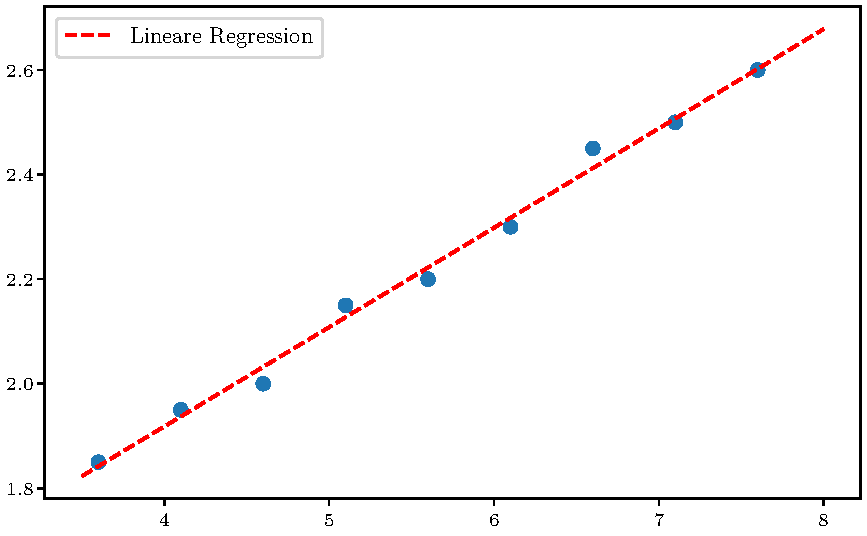
\includegraphics{plot1.pdf}
    \caption{Benötigte Stromstärke in Abhängigkeit zum Abstand zur Kugel.}
    \label{fig:grav}
\end{figure}
Da entsprechend gelten muss, dass
\begin{align}
    & a_1=\frac{2m_rg\left(R^2+\left(\frac{d}{2}\right)^2\right)^\frac{3}{2}}{\mu_0N|\vec{m}|R^2} \\
    \iff & |\vec{m}|=\frac{2m_rg\left(R^2+\left(\frac{d}{2}\right)^2\right)^\frac{3}{2}}{\mu_0NR^2a_1}
\end{align}
ist ergibt sich bei einem Wert für $m_r=\qty{1.4}{\gram}$, dass $|\vec{m}_G|=\qty{0.533(0.017)}{\ampere\meter\squared}$ ist.

\subsection{Schwingungsdauer Methode}

\begin{table}[H]
  \centering
  \caption{Die 10-fache Schwingungsdauer bei einer gegebenen Stromstärke}
  \label{tab:schwing}
  \begin{tblr}{
    colspec={S S},
    row{1}={guard, mode=math},}
    \toprule
    I\mathbin{/}\unit{\ampere}  & 10T\mathbin{/}\unit{\second} \\
    \midrule
    1.5  &   23.04\\
    1.7  &   19.34\\
    1.9  &   17.53\\
    2.1  &   15.50\\
    2.3  &   14.10\\
    2.5  &   13.16\\
    2.7  &   12.88\\
    2.9  &   11.75\\
    3.1  &   11.41\\
    3.3  &   11.03\\
    \bottomrule
  \end{tblr}
\end{table}
Zur Bestimmung des magnetischen Dipolmoments mithilfe der Schwingungsdauer wird Gleichung \ref{eqn:schwingdauer2} betrachtet.
Hier wird erneut eine lineare Regression durchgeführt, in der $\frac{1}{B}$ gegen $T^2$ betrchtet wird, wobei $B$ hier wieder
mithilfe von Gleichung \ref{eqn:magfeld} bestimmt wird. Also sieht die Regression hier so aus $T^2=a_2\frac{1}{B}+b_2$.
\begin{figure}[H]
  \centering
  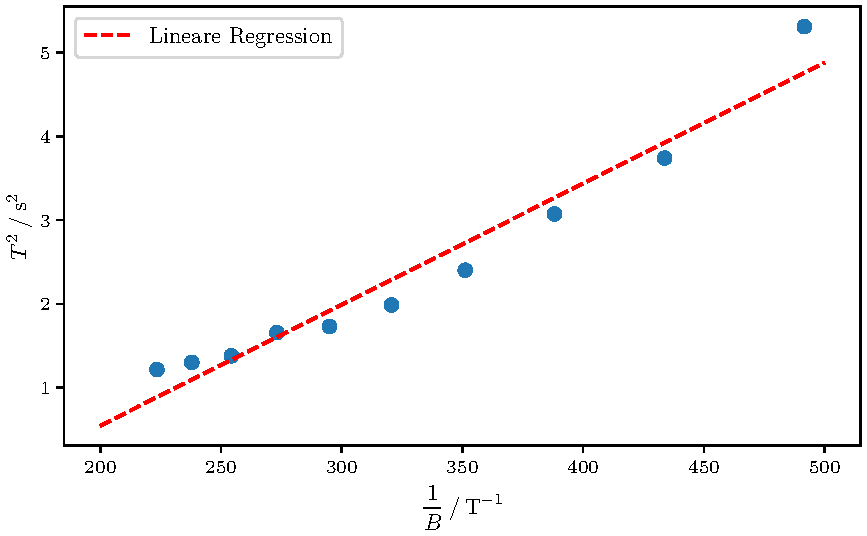
\includegraphics{plot2.pdf}
  \caption{Schwingungsdauer der Kugel in Abhängigkeit der Stromstärke.}
  \label{fig:schwing}
\end{figure}
Hierbei betragen $a_2=\qty{0.101(0.008)}{\tesla\second\squared}$ und $b_2=\qty{-2.3(0.4)}{\second\squared}$.
Durch Vergleich mit Gleichung \ref{eqn:schwingdauer2} geht hervor, dass 
\begin{align}
  &a_2=\frac{4\pi^2J_K}{|\vec{m}|}\\
  \iff &|\vec{m}|=\frac{4\pi^2J_K}{a_2}
\end{align}
ist. Also ist $|\vec{m_S}|=\qty{0.101(0.008)}{\ampere\meter\squared}$.